\section{Segment coordinate transform}

For the following calculations we define the following points of the wing segment: $\vec p_1$ is the innermost point of the leading edge, $\vec p_2$ the outermost point of the leading edge, $\vec p_3$ the innermost point of the trailing edge, and $\vec p_4$ the outermost point of the trailing edge.

\begin{figure}[htb]
  \centering
  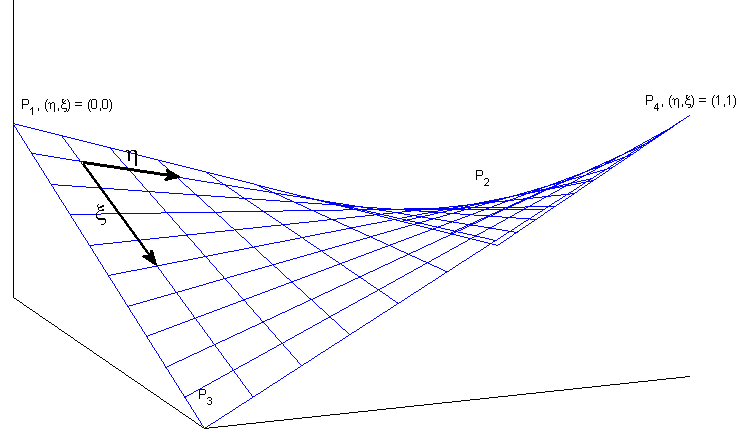
\includegraphics[width = 10cm]{gfx/bilinearSurface}
	\caption{Mathematically, a the chord face of a wing segment is a bilinear surface}
	\label{fig:bilin_surf}
\end{figure}

\subsection{Parametrization of the chord surface}

For simplicity, lets rename $\alpha := \eta$, $\beta := \xi$. Each point $\vec p$ on the surface then be expressed by

\begin{align}
\vec p(\alpha, \beta) &= \left( \vec {p_1} (1-\alpha) + \vec {p_2} \alpha \right) (1-\beta) \\
                  &+ \left( \vec {p_3} (1-\alpha) + \vec {p_4} \alpha \right) \beta \\
                  &= \alpha \underbrace{(-\vec p_1 + \vec p_2)}_{\vec a} + \beta\underbrace{(-\vec p_1 + \vec p_3)}_{\vec b} + \alpha \beta \underbrace{(\vec p_1 - \vec p_2 - \vec p_3 + \vec p_4)}_{\vec c} + \underbrace{\vec p_1}_{\vec d}
\label{eq:param}
\end{align}

This formula defines the transformation between the segments coordinates $(\alpha, \beta)$ to cartesian coordinates $(x, y, z)$. Mathematically, this form is called called bilinear surface. To sum up:

\begin{align}
\vec p (\alpha, \beta) &= \alpha   \vec a + \beta \vec b + \alpha \beta \vec c + \vec d \, , \quad
\textrm{with}\\
\vec a &= -\vec p_1 + \vec p_2 \nonumber \\
\vec b &= -\vec p_1 + \vec p_3 \nonumber \\
\vec c &= \vec p_1 - \vec p_2 - \vec p_3 + \vec p_4 \nonumber \\
\vec d &= \vec p_1 \nonumber
\end{align}

\subsection{Projecting a point onto the chord surface}
The projection of a point $\vec x$ onto the surface is defined as the point $\vec p(\alpha, \beta)$ so that $\vec p (\alpha, \beta) - \vec x$ is orthogonal to the surface. Mathematically it can be shown, that the orthogonality requirement is equivalent to finding the point $\vec p(\alpha, \beta)$ that has a smallest distance to $\vec x$. \par
This is of course an optimization problem which can be defined as:
\begin{equation}
\min_{\alpha, \beta} f(\alpha, \beta) := \min_{\alpha, \beta} \Vert \vec p(\alpha, \beta) - \vec x \Vert^2
\end{equation}
This is an almost quadratic problem (it is only quadratic, if $\vec c = 0$) and can be thus solved with Newton's optimization method. Newtons method is an iterative procedure. In our case, we can adapt it as follows:

\begin{algorithm}[htb]
 %\SetAlgoLined
 $(\alpha; \beta)_0 \leftarrow (0; 0)$ \\
 $k \leftarrow 0$\\
 \While{not converged}{
  $(\alpha, \beta)_{k+1} \leftarrow (\alpha, \beta)_{k} - s [\nabla^2 f(\alpha, \beta) ]^{-1} \cdot \vec \nabla f(\alpha, \beta),\quad \textrm{with}\, s \leq 1$\\
  $k \leftarrow k + 1$ \\
 }
 \caption{Newton's optimization algorithm}
\end{algorithm}

 
In order to perform this projection, we need the gradient $\vec \nabla f(\alpha, \beta)$ and the hessian matrix $\nabla^2 f(\alpha, \beta)$, which are defined as the first and second order derivative of $f(\alpha, \beta)$. \\

\paragraph{Gradient}
Using the chain rule, we get for the gradient:
\begin{equation}
\vec \nabla f(\alpha, \beta) = 2 J_p (\alpha, \beta)^T \cdot (\vec p(\alpha, \beta) - \vec x),
\end{equation}
where $J_p (\alpha, \beta)$ is the Jacobian of $\vec p(\alpha, \beta)$. In components this is:
\begin{align}
\frac {\partial f} {\partial \alpha}(\alpha, \beta) &= 2 \left(\frac{\partial \vec p}{\partial \alpha}(\alpha, \beta)\right)^T (\vec p(\alpha, \beta) - \vec x) \nonumber\\
&= 2\left( \vec a + \beta \vec c \right)^T (\vec p(\alpha, \beta) - \vec x) 
\end{align}
and
\begin{align}
\frac {\partial f} {\partial \beta}(\alpha, \beta) &= 2 \left(\frac{\partial \vec p}{\partial \beta}(\alpha, \beta)\right)^T (\vec p(\alpha, \beta) - \vec x) \nonumber\\
&= 2\left( \vec b + \alpha \vec c \right)^T (\vec p(\alpha, \beta) - \vec x) 
\end{align}

\paragraph{Hessian}
A derivative of the gradient gives as the Hessian matrix:
\begin{align}
\nabla^2 f(\alpha, \beta) = 2 J_p (\alpha, \beta)^T J_p (\alpha, \beta) + 2 (\nabla^2 \vec p (\alpha, \beta))^T \cdot (\vec p(\alpha, \beta) - \vec x)
\end{align}
Thus for the diagonal elements of the Hessian, we get
\begin{align}
\frac {\partial^2 f} {\partial \alpha^2}(\alpha, \beta) &= 2(\vec a + \beta \vec c)^T(\vec a + \beta \vec c) = 2 \Vert \vec a + \beta \vec c \Vert^2 \\
\frac {\partial^2 f} {\partial \beta^2}(\alpha, \beta) &= 2(\vec b + \alpha \vec c)^T(\vec b + \alpha \vec c) = 2 \Vert \vec b + \alpha \vec c \Vert^2 
\end{align}
and for the off-diagonals
\begin{align}
\frac {\partial^2 f} {\partial \alpha \partial  \beta}(\alpha, \beta) 
&= 2(\vec a + \beta \vec c)^T(\vec b + \alpha \vec c) + 2(\vec p (\alpha, \beta) - \vec x)^T \vec c.
\end{align}
Due to the symmetry of the Hessian, we get the same result for the other off-diagonal element $\frac {\partial^2 f} {\partial \beta \partial  \alpha}(\alpha, \beta)$.